%!TEX root = ../thesis.tex

\chapter{Experiments} % Main chapter title

\label{chapter:Experiments} % Change X to a consecutive number; for referencing this chapter elsewhere, use \ref{ChapterX}

\lhead{Chapter 10 \emph{Experiments}} % Change X to a consecutive number; this is for the header on each page - perhaps a shortened title
As previously said, we implemented five experiments : three are based on our graph structure and two directly use the content of Wikipedia's pages. We will now present the dataset we used, the experiments' implementation, the results we obtained and discuss them.

\section{Dataset} % (fold)
\label{sec:dataset}
Our experiments have been made using a database of images pulled out the website Flickr\footnote{https://www.flickr.com/} by fellow students\footnote{Thanks to Adela Neacsu, Sorana Capalnean, Iler Viraragavane and Gaëtan Deshayes}. Some statistics about the database are presented in Table \ref{table:db_stats}.\\
\begin{table}[!h]
\centering
\begin{tabular}{|c|c|c|}
\hline
{\bf Nb. of images} & {\bf Distinct unique tags} & {\bf Avg. nb. of initial tags} \\ \hline
55600               & 10261                      & 17.69                          \\ \hline
\end{tabular}
\caption{Database statistics}
\label{table:db_stats}
\end{table}

\newpage

The top 20 used tags are also available below.
\begin{multicols}{2}
\begin{enumerate}
  \item photography : 55002
  \item colour image : 49734
  \item outdoors : 49129
  \item no people : 44892
  \item day : 37337
  \item sky : 23964
  \item travel destinations : 17713
  \item cloud : 16906
  \item tree : 12890
  \item scenics : 12134
  \item tranquility : 11668
  \item tranquil scene : 10526
  \item landscape : 10303
  \item building exterior : 9941
  \item beauty in nature : 9686
  \item people : 8198
  \item sea : 8197
  \item capital cities : 8144
  \item close-up : 8083
  \item reflection : 7393
\end{enumerate}
\end{multicols}

For the purpose of our tests, we created a graph based on 1350 images that are located around Berlin (Germany). The PostgreSQL query we used to extract them is available in Code \ref{code:berlin}.
\lstinputlisting[language=SQL,caption=PostgreSQL query to retrieve images around Berlin,label={code:berlin}]{./Primitives/berlinImages.sql}

This gave us a graph which contains 5212 nodes and 7543 relations, their distributions are presented in Tables \ref{table:nodes} and \ref{table:edges}. An example of a Cypher query counting the WordNet's nodes is also presented in Code \ref{code:cypherWordNet}.\\

\begin{table}[!h]
\centering
\begin{tabular}{|c|c|c|c|}
\hline
{\bf Virtual} & {\bf Base} & {\bf WordNet} & {\bf DBpedia} \\ \hline
2             & 1619       & 2613          & 978           \\ \hline
\end{tabular}
\caption{Nodes' types distribution}
\label{table:nodes}
\end{table}

\begin{table}[!h]
\centering
\begin{tabular}{|c|c|c|}
\hline
{\bf VIRTUAL} & {\bf PARENT} & {\bf EQUIV} \\ \hline
1612          & 3592         & 2339      \\ \hline
\end{tabular}
\caption{Edges' types distribution}
\label{table:edges}
\end{table}

\lstinputlisting[language=SQL,caption=Cypher query to count WordNet's nodes,label={code:cypherWordNet}]{./Primitives/wordNetCypher.sql}

Thanks to the Gephi software\footnote{http://gephi.github.io/}, we were able to compute some statistics about our network and we learned that the longest shortest path between two nodes (also called graph's diameter) of our graph is of 20 and the average path length between two nodes is of 6.64.

% section dataset (end)
\section{Computer Characteristics} % (fold)
\label{sec:computer_characteristics}
The computer we will use for our operations has the following characteristics :
\begin{enumerate}
  \item OS : Ubuntu 14.04 LTS (64 bits)
  \item RAM : 3,7 Go
  \item CPU : Intel Celeron(R) CPU 847 @ 1.10GHz x 2
\end{enumerate}
% section computer_characteristics (end)

\section{Algorithms Explanation}
The algorithms we will present in this section are supported by the experiments classes we detailed in \ref{sub:semobsneo4j}.

\subsection{Matrices exports} % (fold)
\label{sub:matrices_exports}
As presented in \ref{sub:semobsneo4j}, we developed a way to calculate semantic distances between nodes and export the results as matrices. To achieve this, we implemented two measures : the Shortest Path distance (see \ref{ssub:shortest_path}) and the evolved Wu-Palmer algorithm (see \ref{ssub:evolved_wu_palmer}). This last implementation also implies the development of a Cypher query which retrieves two nodes' LCS. See Code \ref{code:lca} for the complete query.\\
\lstinputlisting[language=SQL,caption=Cypher query to retrieve two nodes' LCS,float,label={code:lca}]{./Primitives/lcaCypher.sql}

With our architecture, it is possible to compute a distance matrix for each image based on its initial tags or to compute a bigger and global matrix taking all images' tags into account.\\

These exports are a support to the comparison of our implemented semantic distances and other metrics one would like to use, like the statistical matrices produced by the tool presented in \ref{sec:statistical_similarity}.\\

The computation of such matrices cost around 20 seconds for 15 tags on the machine presented in \ref{sec:computer_characteristics}.
% subsection matrices_exports (end)

\subsection{Graph-based experiments} % (fold)
\label{sub:graph_based_experiments}
The two first experiments, WholeList (short WL) and SubLists (short SL), are based on the same algorithm of candidates detection. This algorithm make use of Breadth-First search (BFS) traversers in order to browse the graph starting from the initial tags' nodes. The BFS implementation is available on Code \ref{code:bfs} and the candidates detection algorithm on Code \ref{code:newtags}.\\
\lstinputlisting[language=Java,caption=Java BFS implementation,float,label={code:bfs}]{./Primitives/BFS.java}
\lstinputlisting[language=Java,caption=Candidates detection algorithm,float,label={code:newtags}]{./Primitives/newTags.java}
\subsubsection{Lists - WL} % (fold)
\label{ssub:lists_wl}
The difference between WL and SL is located line 26 of Code \ref{code:newtags} : the score computation function doesn't take the same things into account. Let's detail this.\\
In the WL experiment, we compute a global score using all the initial tags (Whole List). This global score is composed of all the scores between the considered candidate and the initial nodes as follows :
\begin{equation}
\label{eq:wholeList}
globalScore(currentNode) = \sum_{0\le n< nbNodes} \frac{1}{score(currentNode, nodes(n))^k}
\end{equation}
The $score$ function can be one of the measures we presented in \ref{chapter:Measures}. Due to computer performances we had to go with the Shortest Path distance. $k$ is a chosen integer which has for consequence to favor (or not) really close nodes.
% subsubsection lists_wl (end)
\subsubsection{Lists - SL} % (fold)
\label{ssub:lists_sl}
The SL experiment is based on the same approach than his brother WL. The difference is that, when it comes to global score computing, we only take into account a determined number of initial nodes. This results on a small modification of the algorithm : before any global score calculation we store all the $score$ results and only use some of them in equation \eqref{eq:wholeList}. This has for consequence that the very far nodes don't pollute our results by inserting noise. 
% subsubsection lists_sl (end)\subsubsection{Direct Neighbors}
\subsubsection{Direct Neighbors} % (fold)
\label{ssub:direct_neighbors}
This last graph-based experiment version is more direct : we search for direct neighbors of the input nodes. In concrete terms, for each of the input nodes, we store all the parents nodes with a maximal distance of 2. We count how many times each parent is found and return the most frequent ones. This method is expected to give good results when the initial tags are close semantically speaking (boat, sea, sail \dots) but can return abstract results in the case of a very diverse set of tags, and even more if this set is small.
% subsubsection direct_neighbors (end)
% subsection graph_based_experiments (end)
\subsection{Plain-text experiments} % (fold)
\label{sub:plain_text_experiments}
We will now present the last two experiments which are directly based on the content of Wikipedia's pages, extracted with the help of the JSoup library (see \ref{sub:jsoup}). The process is basically the same : we search for wikipedia's pages matching the URL \emph{https://en.wikipedia.org/wiki/+TAG}, if found we extract the content from the first paragraph and then operate the candidate detection step.
\subsubsection{WikiLinks} % (fold)
\label{ssub:wikilinks}
For the WikiLinks experiment, we only care about internal links (called wikilinks). We access them using CSS queries :
\begin{itemize}
	\item Access the 1st paragraph : \emph{div\#mw-content-text $>$ p}
	\item Access wikilinks : \emph{a[href~=/wiki/(?!Help:)(?!File:)(?!Wikipedia:)]}
\end{itemize}
Here again, we store each of the links and sum its occurrences, we then propose as final candidates the most frequent ones.
% subsubsection wikilinks (end)
\subsubsection{WikiContent} % (fold)
\label{ssub:wikicontent}
The WikiContent experiment is very similar to the WikiLinks one. The difference is that we consider here all the nouns in the first paragraph of the Wikipedia's page. In order to achieve this, we extract the first paragraph with the same CSS query presented above and then parse its content using the NLP library. The Part-of-speech module gives us a list of tokens as well as their POS label (see below for the complete list of POS labels) and we then only keep the nouns (NN* labels : common and proper nouns, singular and plural).\\
Here again, we store each of the links and sum its occurrences, we then propose as final candidates the most frequent ones.
\begin{multicols}{2}
\begin{itemize}
  \item CC Coordinating conjunction
  \item CD Cardinal number
  \item DT Determiner
  \item EX Existential there
  \item FW Foreign word
  \item IN Preposition or subordinating conjunction
  \item JJ Adjective
  \item JJR Adjective, comparative
  \item JJS Adjective, superlative
  \item LS List item marker
  \item MD Modal
  \item NN Noun, singular or mass
  \item NNS Noun, plural
  \item NNP Proper noun, singular
  \item NNPS Proper noun, plural
  \item PDT Predeterminer
  \item POS Possessive ending
  \item PRP Personal pronoun
  \item PRP\$ Possessive pronoun
  \item RB Adverb
  \item RBR Adverb, comparative
  \item RBS Adverb, superlative
  \item RP Particle
  \item SYM Symbol
  \item TO to
  \item UH Interjection
  \item VB Verb, base form
  \item VBD Verb, past tense
  \item VBG Verb, gerund or present participle
  \item VBN Verb, past participle
  \item VBP Verb, non 3rd person singular present
  \item VBZ Verb, 3rd person singular present
  \item WDT Whdeterminer
  \item WP Whpronoun
  \item WP\$ Possessive whpronoun
  \item WRB Whadverb
\end{itemize}
\end{multicols}
% subsubsection wikicontent (end)
% subsection plain_text_experiments (end)

\section{Results and Analysis} % (fold)
\label{sec:results_and_analysis}
\subsection{Evaluation methodology} % (fold)
\label{sub:evaluation_methodology}
Now that we have presented our experiments, we will explain how we evaluated them using two different methods.\\

The first one only applies to the three graph-based experiments : we were able to compute a distance metric between a removed percentage (30\%) of the initial tags and the candidates. This distance is based on the Shortest Path metric and take all kinds and directions of edges into account.\\

The second method is an user-based evaluation, we asked several individuals to rate the generated candidates regarding the image and the initial tags.\\

% subsection evaluation_methodology (end)

\subsection{Evaluation results} % (fold)
\label{sub:evaluation_results}
\subsubsection{Semantic distance average} % (fold)
\label{ssub:semantic_distance_average}
We ran our tests on 100 images among those used to create our graph. All of the considered images have a minimum set of initial tags of at least 7 items. The three experiments (WL, SL and DN) were used on each image and we computed the distance metric for each of them. Eventually, we calculated the average distance for each experiment. The results are presented in Table \ref{table:avgDist}.\\
\begin{table}[!h]
\centering
\begin{tabular}{ccc}
\cline{1-3}
\multicolumn{1}{|c|}{{\bf WholeList}} & \multicolumn{1}{c|}{{\bf Sub-Lists}} & \multicolumn{1}{c|}{{\bf Direct Neighbors}} \\ \cline{1-3}
\multicolumn{1}{|c|}{3.95}     & \multicolumn{1}{c|}{3.90}     & \multicolumn{1}{c|}{3.55} \\ \cline{1-3}
\end{tabular}
\caption{Average distance between removed tags and candidates}
\label{table:avgDist}
\end{table}

We observe that the DN experiment has better results than the list-based ones. These are really close and this can be explained by the fact that their candidates are often the same but in a different order. These results are pretty good since our diameter (ie the longest shortest path between two nodes in our graph) is of 20. The EQUIV edges are certainly helping these results : without them, the shortest path between a base node which only has generalizations in the WordNet's ontology and one which only has its in the DBpedia's ontology would inevitably contain the virtual root node. This would make the distances way more longer.\\

The computation of these results cost around 1.5 hour for 100 images.
% subsubsection semantic_distance_average (end)
\subsubsection{User evaluation} % (fold)
\label{ssub:user_evaluation}
For this method, we also used 100 images with a minimum amount of initial tags of 7, ran all experiments for each image and stored all the results. Then we generated lots with the following rules :
\begin{itemize}
  \item Each lot only concern one type of test (WL, SL, DN, WikiLinks or WikiContent)
  \item Each lot contains the chosen test's results for 5 images
  \item Each test is evaluated by several people
  \item Each lot is sent to several people
\end{itemize}

The next step was to send the lots to our testers. They were mainly engineering students from INSA Lyon but only 27\% of them study computer science. They were given a HTML file with 5 images to evaluate (see Figure \ref{fig:userEval} for an example of one) and a CSV file to write their evaluation. The question they had to answer was \emph{Does this tag describe the image ?} and they had to rate each tag on a scale of 1 (\emph{Strongly Agree}) to 5 (\emph{Strongly Disagree}) with an \emph{Undecided} option (3). As already said, each person only evaluated one experiment (WL, SL, DN, WikiLinks or WikiContent) and each experiment was evaluated by different people. We concatenated the results and computed several statistics presented in Table \ref{table:userEval}.\\

\begin{figure}
  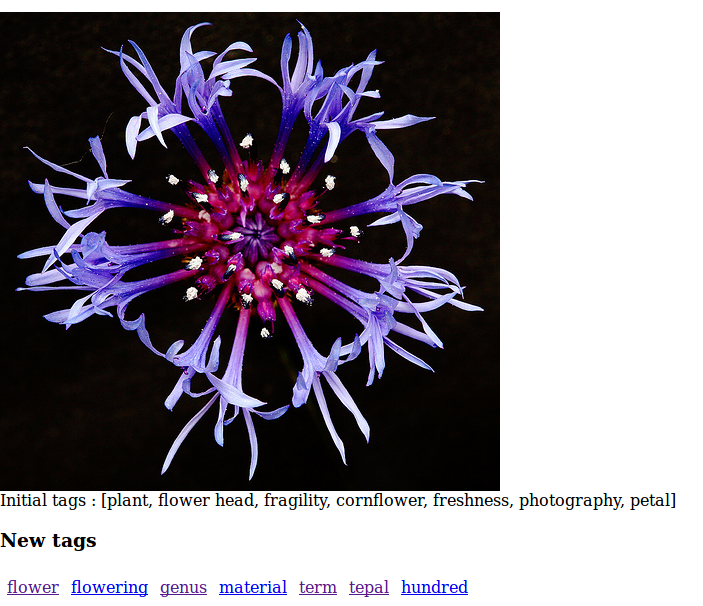
\includegraphics[scale=0.6]{./Primitives/exampleEval}
  \caption{User-evaluation sample}
  \label{fig:userEval}
\end{figure}

\begin{table}[!h]
\centering
\begin{tabular}{|l|c|c|c|c|c|}
\hline
{\bf } & {\bf WL} & {\bf SL} & {\bf DN} & {\bf WikiLinks} & {\bf WikiContent} \\ \hline
{\bf Avg.  global rating} & 3.30 & 3.29 & 3.09 & 3.25 & 2.55 \\ \hline
{\bf Avg. 1st candidate rating} & 2.70 & 2.33 & 2.73 & 3.13 & 1.93 \\ \hline
{\bf Avg. 2nd candidate rating} & 3.45 & 2.96 & 3.6 & 2.67 & 2.19 \\ \hline
{\bf Avg. 3rd candidate rating}  & 3.15 & 3.33 & 3.13 & 2.53 & 2.82 \\ \hline
\end{tabular}
\caption{User-evaluation results}
\label{table:userEval}
\end{table}

These results are interesting, it is very clear that the WikiContent experiment is the best and among the graph-based ones, the DN experiment seems to be the more promising. We also wanted to see if the theory in which the firsts tags are the better ones was correct, and we can't really conclude anything based on these results since no rule seems to apply (only SL and WikiContent follow this pattern). However, it is nice to see that the first tag is almost always the best tag (only WikiLinks refute this). In average, the global rating is around 3, which isn't bad but isn't so good as well. More has to be done in order to enhance our prototype and perspectives are presented in the next chapter.

% subsubsection user_evaluation (end)
% subsection evaluation_results (end)
% section results_and_analysis (end)
